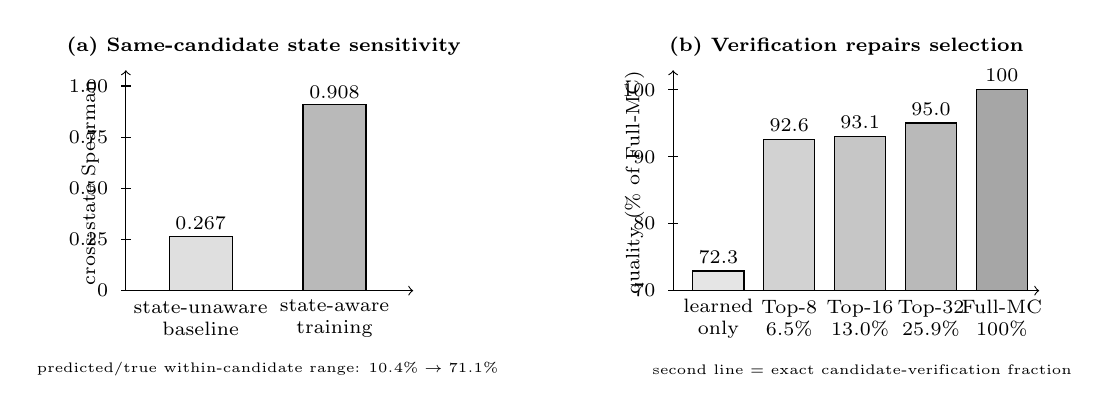
\begin{tikzpicture}[font=\scriptsize]
% Panel (a): state awareness
\begin{scope}[xshift=0cm]
  \node[font=\scriptsize\bfseries] at (2.15,3.55) {(a) Same-candidate state sensitivity};
  \draw[->] (0.4,0.45) -- (0.4,3.25);
  \draw[->] (0.4,0.45) -- (4.05,0.45);
  \foreach \y/\lab in {0.45/0,1.10/0.25,1.75/0.50,2.40/0.75,3.05/1.00}{
    \draw (0.34,\y)--(0.46,\y); \node[anchor=east] at (0.30,\y) {\lab};
  }
  \filldraw[fill=gray!25] (0.95,0.45) rectangle (1.75,1.14);
  \filldraw[fill=gray!55] (2.65,0.45) rectangle (3.45,2.81);
  \node at (1.35,1.30) {0.267};
  \node at (3.05,2.97) {0.908};
  \node[align=center] at (1.35,0.10) {state-unaware\\baseline};
  \node[align=center] at (3.05,0.10) {state-aware\\training};
  \node[rotate=90] at (-0.05,1.82) {cross-state Spearman};
  \node[align=center, font=\tiny] at (2.2,-0.55) {predicted/true within-candidate range: $10.4\%\rightarrow71.1\%$};
\end{scope}

% Panel (b): verification repairs sequential selection
\begin{scope}[xshift=7.0cm]
  \node[font=\scriptsize\bfseries] at (2.55,3.55) {(b) Verification repairs selection};
  \draw[->] (0.35,0.45) -- (0.35,3.25);
  \draw[->] (0.35,0.45) -- (5.0,0.45);
  \foreach \y/\lab in {0.45/70,1.30/80,2.15/90,3.00/100}{
    \draw (0.29,\y)--(0.41,\y); \node[anchor=east] at (0.25,\y) {\lab};
  }
  \def\base{0.45}
  % height mapping: y=0.45 + (quality-70)*0.085
  \filldraw[fill=gray!20] (0.60,0.45) rectangle (1.25,0.70);
  \filldraw[fill=gray!35] (1.50,0.45) rectangle (2.15,2.37);
  \filldraw[fill=gray!45] (2.40,0.45) rectangle (3.05,2.41);
  \filldraw[fill=gray!55] (3.30,0.45) rectangle (3.95,2.58);
  \filldraw[fill=gray!70] (4.20,0.45) rectangle (4.85,3.00);
  \node at (0.925,0.88) {72.3};
  \node at (1.825,2.55) {92.6};
  \node at (2.725,2.59) {93.1};
  \node at (3.625,2.76) {95.0};
  \node at (4.525,3.18) {100};
  \node[align=center] at (0.925,0.10) {learned\\only};
  \node[align=center] at (1.825,0.10) {Top-8\\$6.5\%$};
  \node[align=center] at (2.725,0.10) {Top-16\\$13.0\%$};
  \node[align=center] at (3.625,0.10) {Top-32\\$25.9\%$};
  \node[align=center] at (4.525,0.10) {Full-MC\\$100\%$};
  \node[rotate=90] at (-0.14,1.82) {quality (\% of Full-MC)};
  \node[font=\tiny] at (2.75,-0.55) {second line = exact candidate-verification fraction};
\end{scope}
\end{tikzpicture}
